\documentclass[sigconf]{acmart}
\settopmatter{printacmref=false} % Removes citation information below abstract
\renewcommand\footnotetextcopyrightpermission[1]{} % removes footnote with conference information in first column
\pagestyle{plain} % removes running headers

\usepackage{booktabs} % For formal tables


% Copyright
\setcopyright{none}
%\setcopyright{acmcopyright}
%\setcopyright{acmlicensed}
%\setcopyright{rightsretained}
%\setcopyright{usgov}
%\setcopyright{usgovmixed}
%\setcopyright{cagov}
%\setcopyright{cagovmixed}

\settopmatter{printacmref=false}

\usepackage{frame}
\usepackage{tikz}
\def\checkmark{\tikz\fill[scale=0.4](0,.35) -- (.25,0) -- (1,.7) -- (.25,.15) -- cycle;} 
\def\circle{\tikz\draw[scale=0.1] (2,2) circle (1);} 


\begin{document}
\title{Flavor Based Recipe Recommendation}
\subtitle{Team Foodies Progress Report}

\author{Haiyue Yin}
\affiliation{%
  \institution{Georgia Institute of Technology}
  \streetaddress{North Avenue}
  \city{Atlanta} 
  \state{Georgia} 
  \postcode{30332}
}
\email{hyin62@gatech.edu}

\author{Jidong Li}
\affiliation{%
  \institution{Georgia Institute of Technology}
  \streetaddress{North Avenue}
  \city{Atlanta} 
  \state{Georgia} 
  \postcode{30332}
}
\email{jli807@gatech.edu}

\author{Mo Shi}
\affiliation{%
  \institution{Georgia Institute of Technology}
  \streetaddress{North Avenue}
  \city{Atlanta} 
  \state{Georgia} 
  \postcode{30332}
}
\email{mshi61@gatech.edu}

\author{Shan Jing}
\affiliation{%
  \institution{Georgia Institute of Technology}
  \streetaddress{North Avenue}
  \city{Atlanta} 
  \state{Georgia} 
  \postcode{30332}
}
\email{sjing3@gatech.edu}

\author{Sixin He}
\affiliation{%
  \institution{Georgia Institute of Technology}
  \streetaddress{North Avenue}
  \city{Atlanta} 
  \state{Georgia} 
  \postcode{30332}
}
\email{she89@gatech.edu}

\author{Siyi Cao}
\affiliation{%
  \institution{Georgia Institute of Technology}
  \streetaddress{North Avenue}
  \city{Atlanta} 
  \state{Georgia} 
  \postcode{30332}
}
\email{scao34@gatech.edu}


% The default list of authors is too long for headers.
% \renewcommand{\shortauthors}{B. Trovato et al.}


\maketitle

\section{Introduction}
\indent From fire roasting, food preparation has become more than just making raw ingredients more edible. Nowadays people pay more attention to what they eat, and devote much more time in planning for delicious and healthy meals\cite{lansing1920food}.

With the prevalence of online recipe sites such as \textit{Cookpad}, \textit{Allrecipes} and \textit{Yahoo! Recipe}, tremendous amount of recipe data is generated each day \cite{ueda2011user}. This prevalence leads to a growing demand for recipe recommendation systems. 

Here we propose a novel recipe recommendation system that utilizes a combination of factors including user preferences, ingredient frequencies in recipes, and an ingredient flavor network. The goal of this project is to provide an easy-to-use interface that helps users decide on various potential tasty and healthy recipes.

\section{Survey (literature review)}
\textbf{Recommendation Systems}\\
Three strategies are mainly used by recommendation systems: content-based \cite{svensson2000recipe}, collaborative and hybrid systems \cite{sobecki2006application}. However, all of these strategies treat a recipe as an inseparable item \cite{freyne2010intelligent}. Ueda et al. proposed a new recommendation system in which recipes are broken down into quantitative food ingredients, and user's food preferences are considered based on their browsing and cooking history. It was proven to be effective and reasonable to view a recipe as a repository of ingredient combinations and cooking methods \cite{ueda2011user}\cite{ueda2014recipe}.

There are some proposed problems of users’ rating for recommendation system, such as the cold-start problem \cite{bobadilla2013recommender} and biased ratings\cite{rokicki2017editorial}. Although Bayesian classifier may solve the cold-start problem \cite{miyahara2000collaborative}, we still need to make good use of users rating more carefully.\\
\indent Recipe recommendation may consider a range of factors. Bianchini et al. consider prescription information as a key role for menu recommendation \cite{bianchini2017prefer}. Both Karikome et al. and Ueta et al. try to make nutrition a key factor for their recommendation systems \cite{karikome2010system}\cite{ueta2011recipe}.\\


\hfill \break

\noindent
\textbf{Food Pairing and Bridging}\\
However, flavor is rarely addressed in the systems mentioned above. Food flavor is the main sensory property that influences food acceptance, and is usually the decisive factor for the choice of a particular product \cite{jelen2011food}.

Various researches have been conducted on the patterns of chemical composition of ingredients in our daily recipes. The food pairing hypothesis states that people tend to put ingredients that share similar flavor compounds together. Ahn et al. also observe that most western cuisines follow the hypothesis by having ingredients that share similar flavors, while eastern cuisines avoid them \cite{ahn2011flavor}\cite{ahn2013flavor}. Simas et al. further show a bridging phenomenon where an intermediate ingredient can smooth ingredients with contrast flavors. They observe that different regions display different combinations of levels of food pairing and food bridging \cite{simas2017food}.

\section{Progress of Proposed Methods}

\noindent
\textbf{Data Collection}\\
Using Spoonacular API we obtained about 50,000 recipes. Then we scraped the flavor information from Fenaroli’s handbook of flavor ingredients.\cite{simas2017food} \cite{burdock2016fenaroli}\\

\noindent
\textbf{Recipe Data Cleaning}\\
The raw recipe data includes structured information such as cuisine type, image link, price, instructions, and a list of complete ingredients wit ID's. The ingredient ID's were not directly availabe since Spoonacular uses a hash function for ingredient ID's. Fortunately Spoonacular's recipe data already contains pre-defined ingredients, and therefore we traversed all the recipes and obtained a list of ingredient ID's with the corresponding lists of ingredients names. Then we used the ingredient list to parse the recipes to obtain ingredient co-occurrences.\\

\noindent
\textbf{Flavor Data Cleaning}\\
This was the most challenging part of data cleaning, since the Fenaroli’s handbook  is in PDF format. We converted it to txt using an online converter, and coarsely parsed the texts using NLP. With a combination of machine and manhours, we obtained a table of the chemical compounds and their corresponding natural occurrences in important ingredient keywords that we named ``essence". We are yet to include the entries of botanic species in the book, which requires further manual processing.\\

\noindent
\textbf{Construction and Integration of Co-occurrence Network and Flavor Network}\\
We matched the essence keywords to the Spoonacular's ingredient names to obtain a mapping between chemical compounds and ingredients. The resulting flavor network is visualized in the visualization section.\\
\indent Assume that we have $n$ recipes and $m$ ingredients which contains $t$ chemical compounds in total. \\
\indent Ingredient occurrence matrix $K$ and flavor compounds matrix $R$ were built to calculate the frequency of each two ingredients occurring in the same recipe and the number of shared chemical compounds between each two ingredient essence. $K_{ij}$ means the $j$th ingredient is used in $i$th recipe or not, with corresponding values of 1 and 0. $R_{ij}$ denotes whether the $j$th ingredient contains $i$th chemical compound. Then we have:
\begin{align*}
K^*=K^\top K \Longrightarrow K^*_{ij}=\sum_{p=1}^n K_{pi}K_{pj} \\
R^*=R^\top R \Longrightarrow R^*_{ij}=\sum_{p=1}^n R_{pi}R_{pj}
\end{align*}
Through the above transformations, we have $K^*_{ij}$ in $K^*$ referring to the number of recipes that contain both the $i$th ingredient and the $j$th ingredient. $R^*_{ij}$ refers to the number of shared compounds between the $i$th ingredient and the $j$th ingredient. \\

\noindent
\textbf{Database Construction and Data Visualization}\\
Databases are built using SQLite3 for various data sets. One of the major table is for all the recipes , and the main data stored for it includes recipe names, ingredients, equipment and steps. Another important table is for storing data of flavor network. It consists by chemical compounds and the corresponding ingredients. Moreover, a co-occurrence table of ingredients is constructed. We used Gephi to visualize the ingredient network as shown below.\\
\begin{center}
\frame{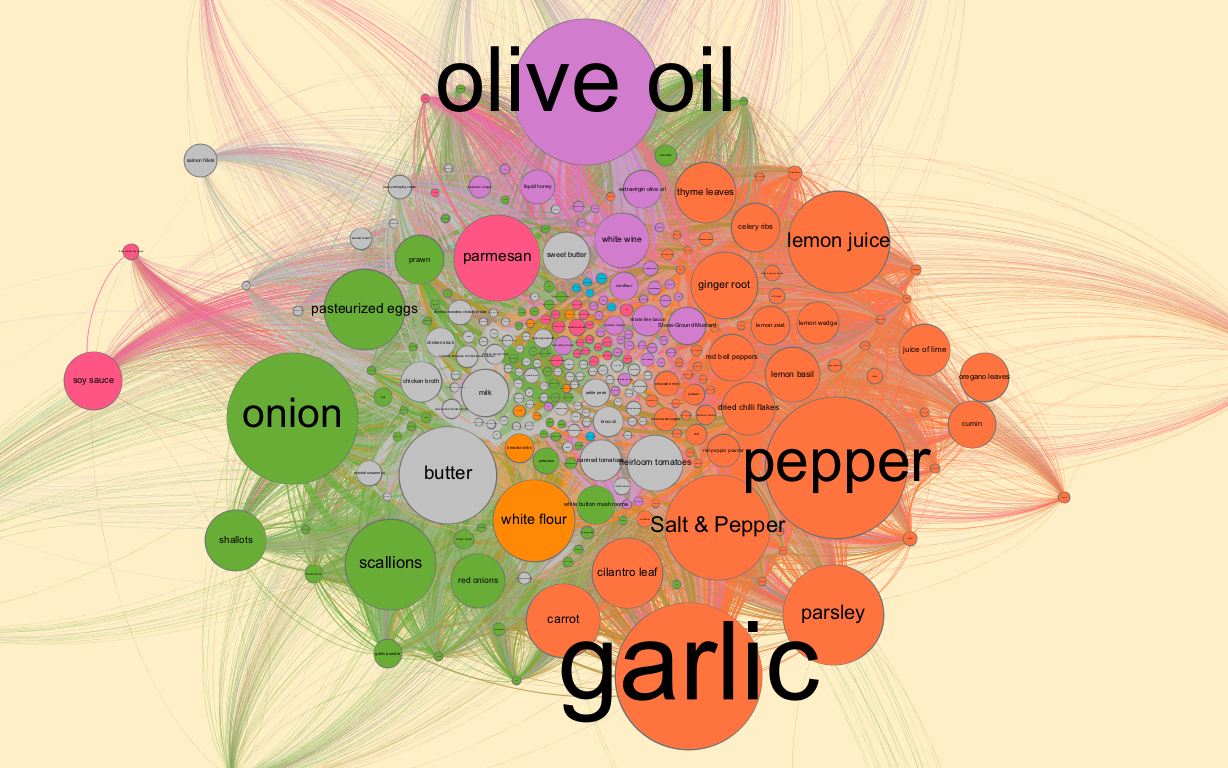
\includegraphics[width=.48\textwidth]{network}}
\end{center}
Above is a visualization of the flavor network. The node size corresponds to the prevalence of the ingredient, and the edge width refers to the number of shared compounds. A simple modularity algorithm was performed on the graph, and one can observer that ingredient with similar flavors tend to be clustered together.\\

\noindent
\textbf{Data Analysis}\\
After we got recipe data, we used Pointwise Mutual Information to get the co-occurrence rate between each two ingredients among our recipes, and use this PMI value to generate an ingredient network. PMI defined on pairs of ingredient (a,b):
\begin{align*}
PMI(a,b)=\log \frac{P(a,b)}{P(a)p(b)}
\end{align*}
where:
\begin{align*}
P(a,b)=\frac{K^*_{ab}}{m} \\
P(a)=\frac{K^*_{aa}}{m} \\
P(b)=\frac{K^*_{bb}}{m}
\end{align*}
The PMI gives the probability that two ingredients occur together against the probability that they occur separately. Complementary ingredients tend to occur together far more often than would be expected by chance.\cite{teng2012recipe}\\

\noindent
\textbf{Recommendation}\\
First, the users will be asked to enter a food ingredient they want to include in their desired recipe. After getting the input ingredient A from the user, a list of ingredients $A^\prime=(A_1^\top,A_2^\top,...,A_n^\top)^\top$ will be found by using the index of PMI in the co-occurrence network sorted in descending order. Then the flavor network is used to filter the list $A^\prime$ by deleting the items who do not share the same chemical compounds with A and find out four top ingredients in $A^\prime$ for users to choose. The selected four ingredients should be those who have relatively high co-occurrences and also share some similar chemical compounds with A. Given the four ingredients, the users will be asked to select several ingredients that they like the most. These ingredients will be further used for recommendation.\\

\noindent
\textbf{Prototype interface}\\
\frame{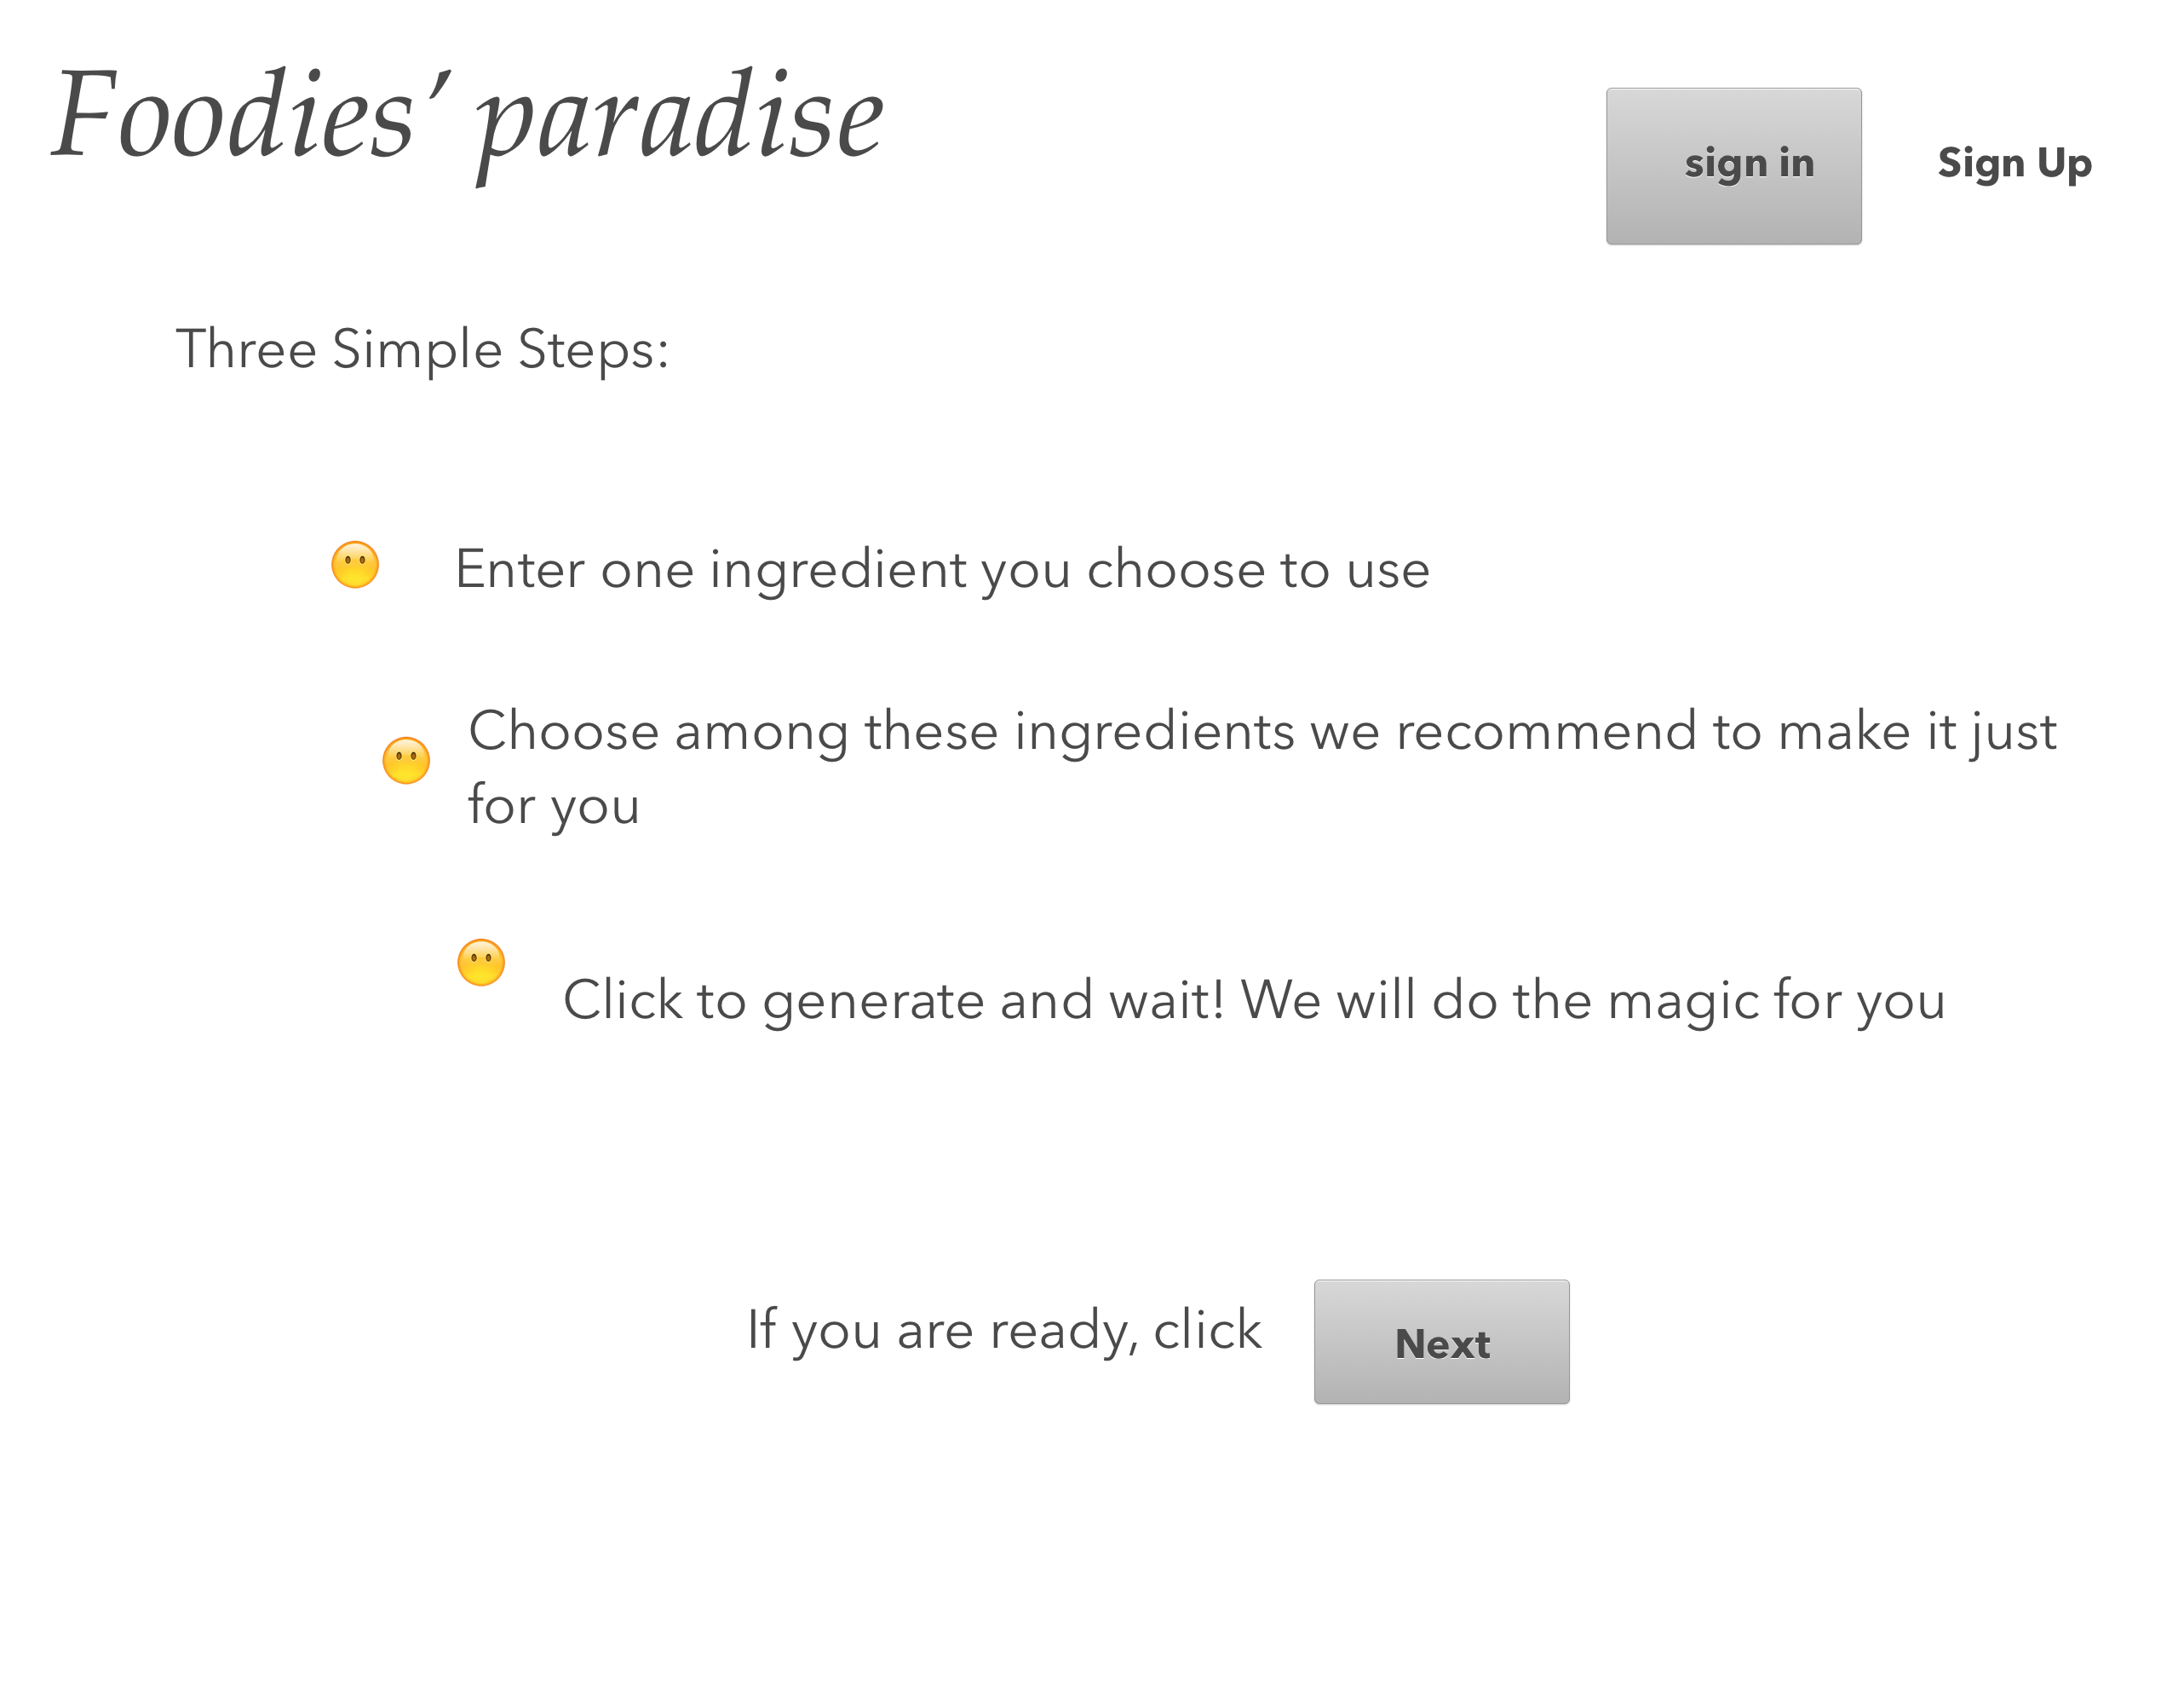
\includegraphics[width=.48\textwidth]{ui_1}} \\
\\
\frame{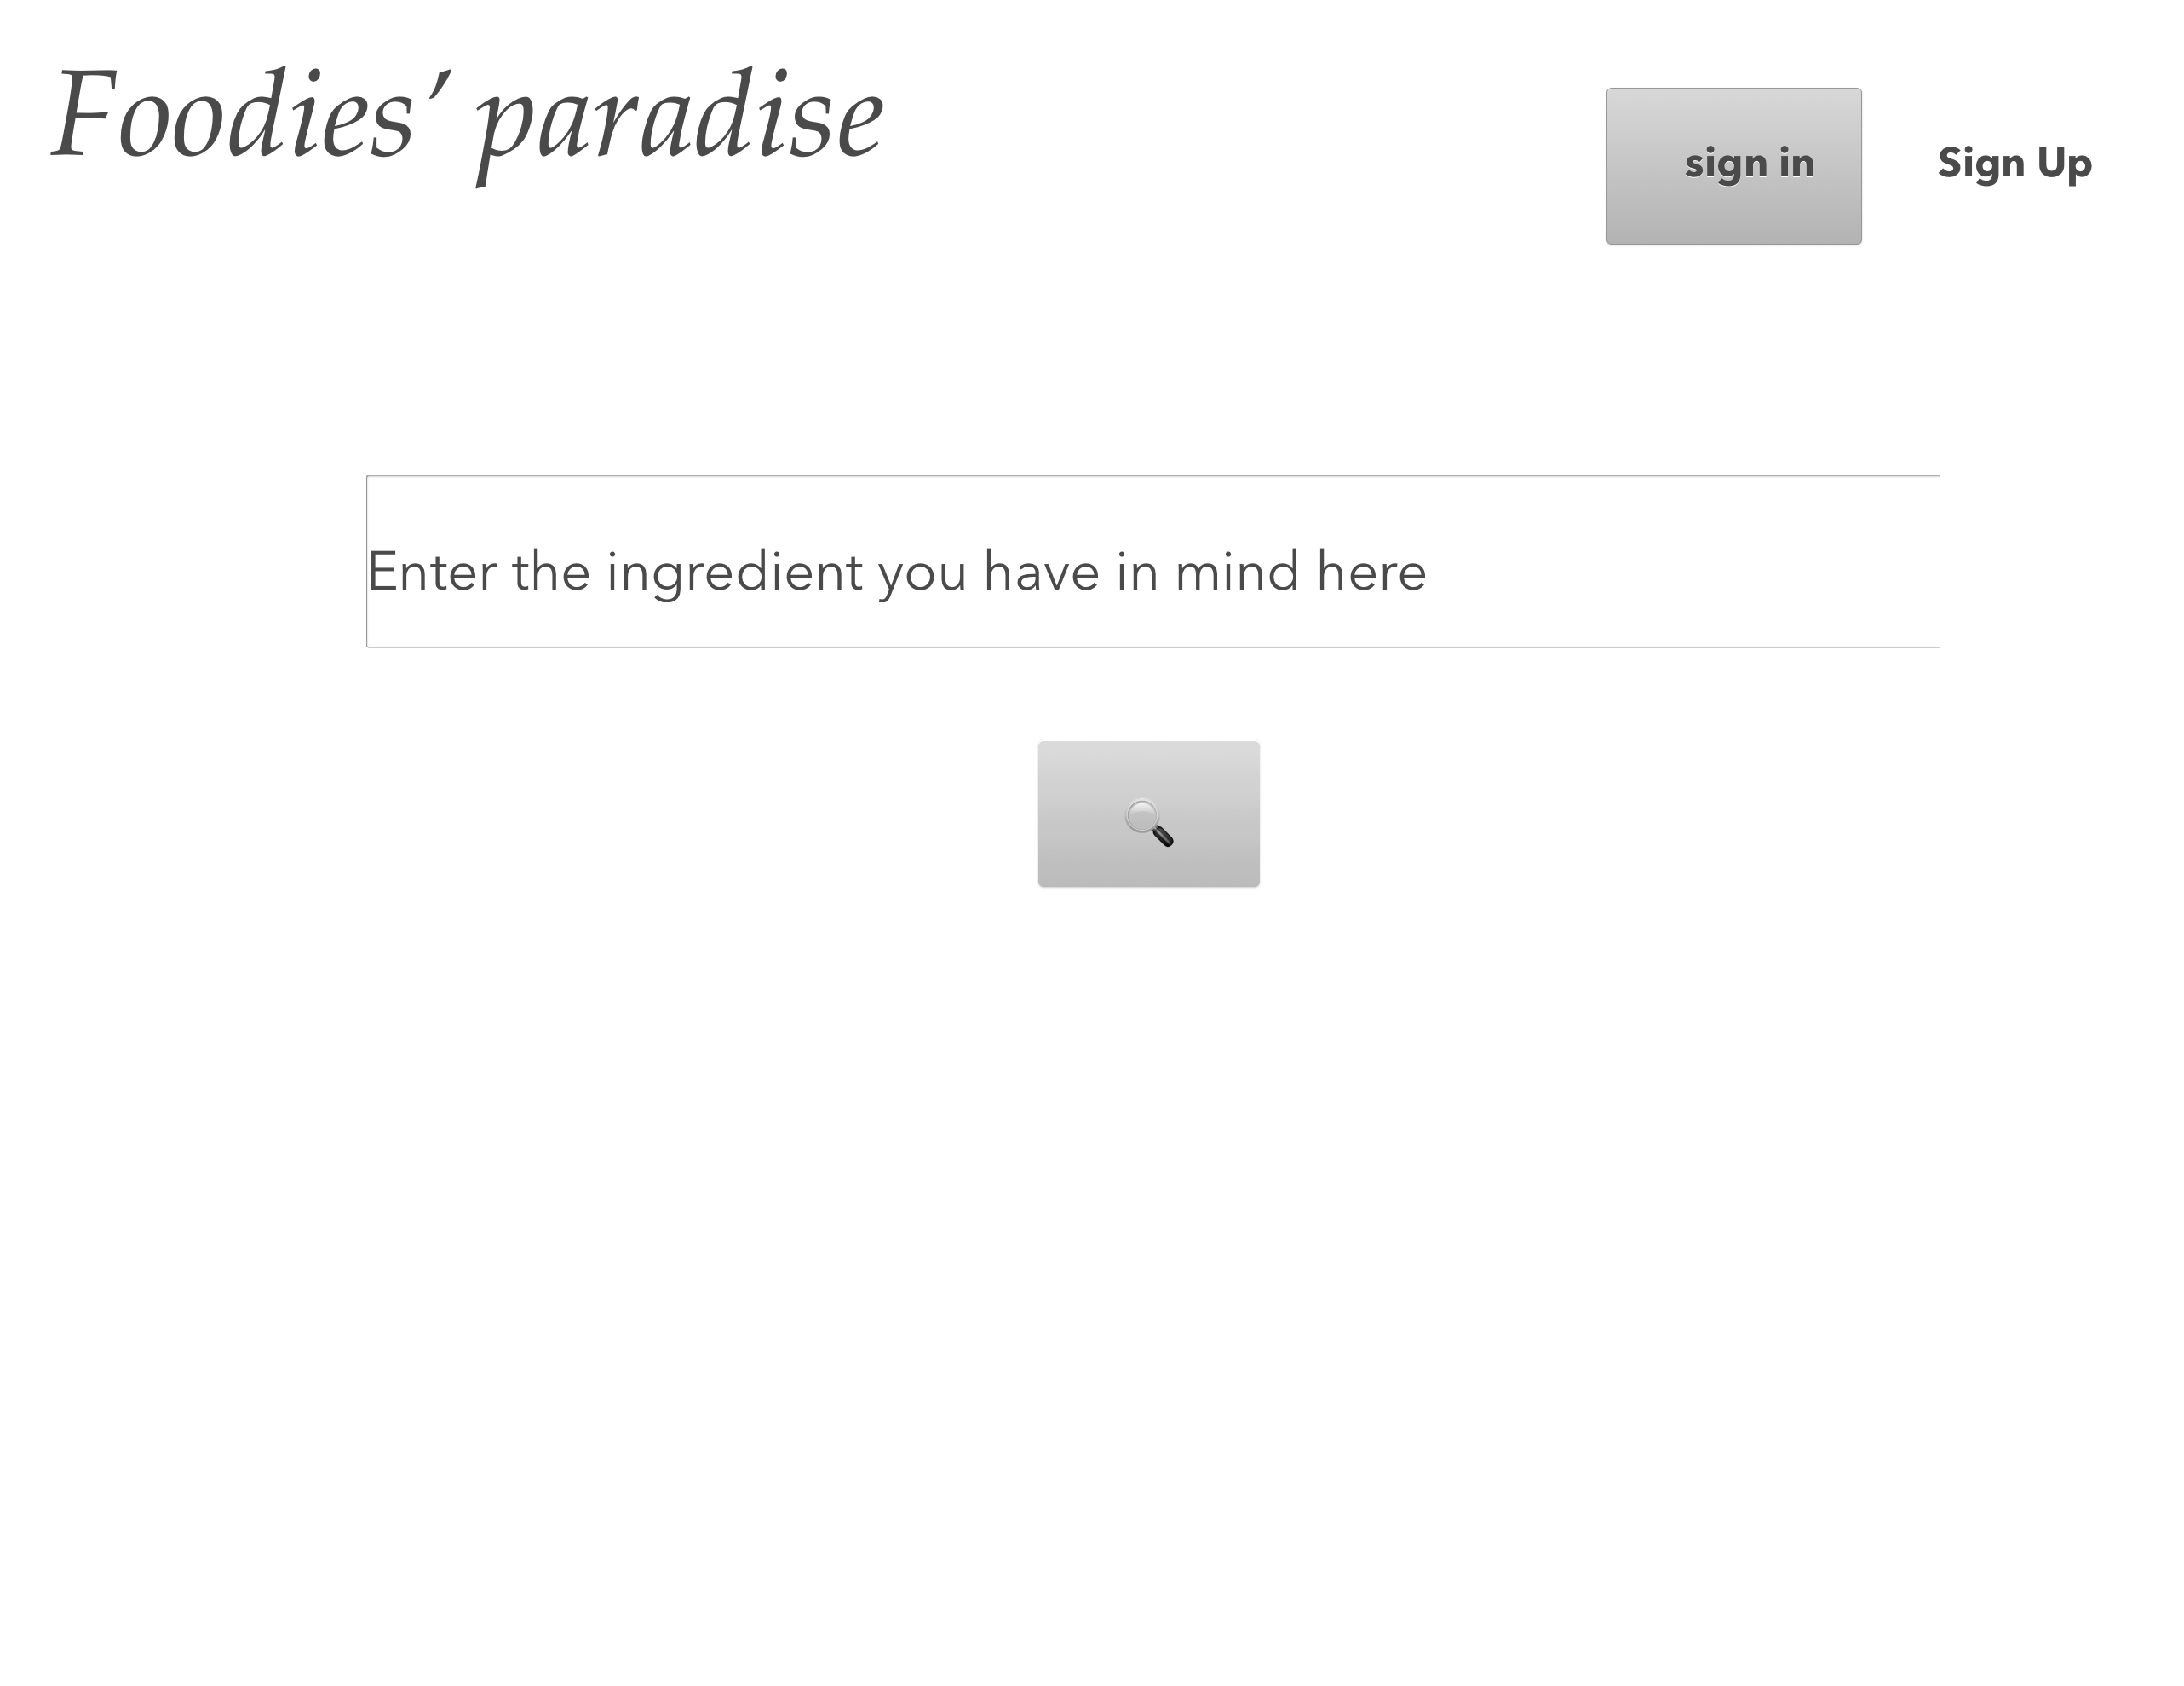
\includegraphics[width=.48\textwidth]{ui_2}} \\
\\
\frame{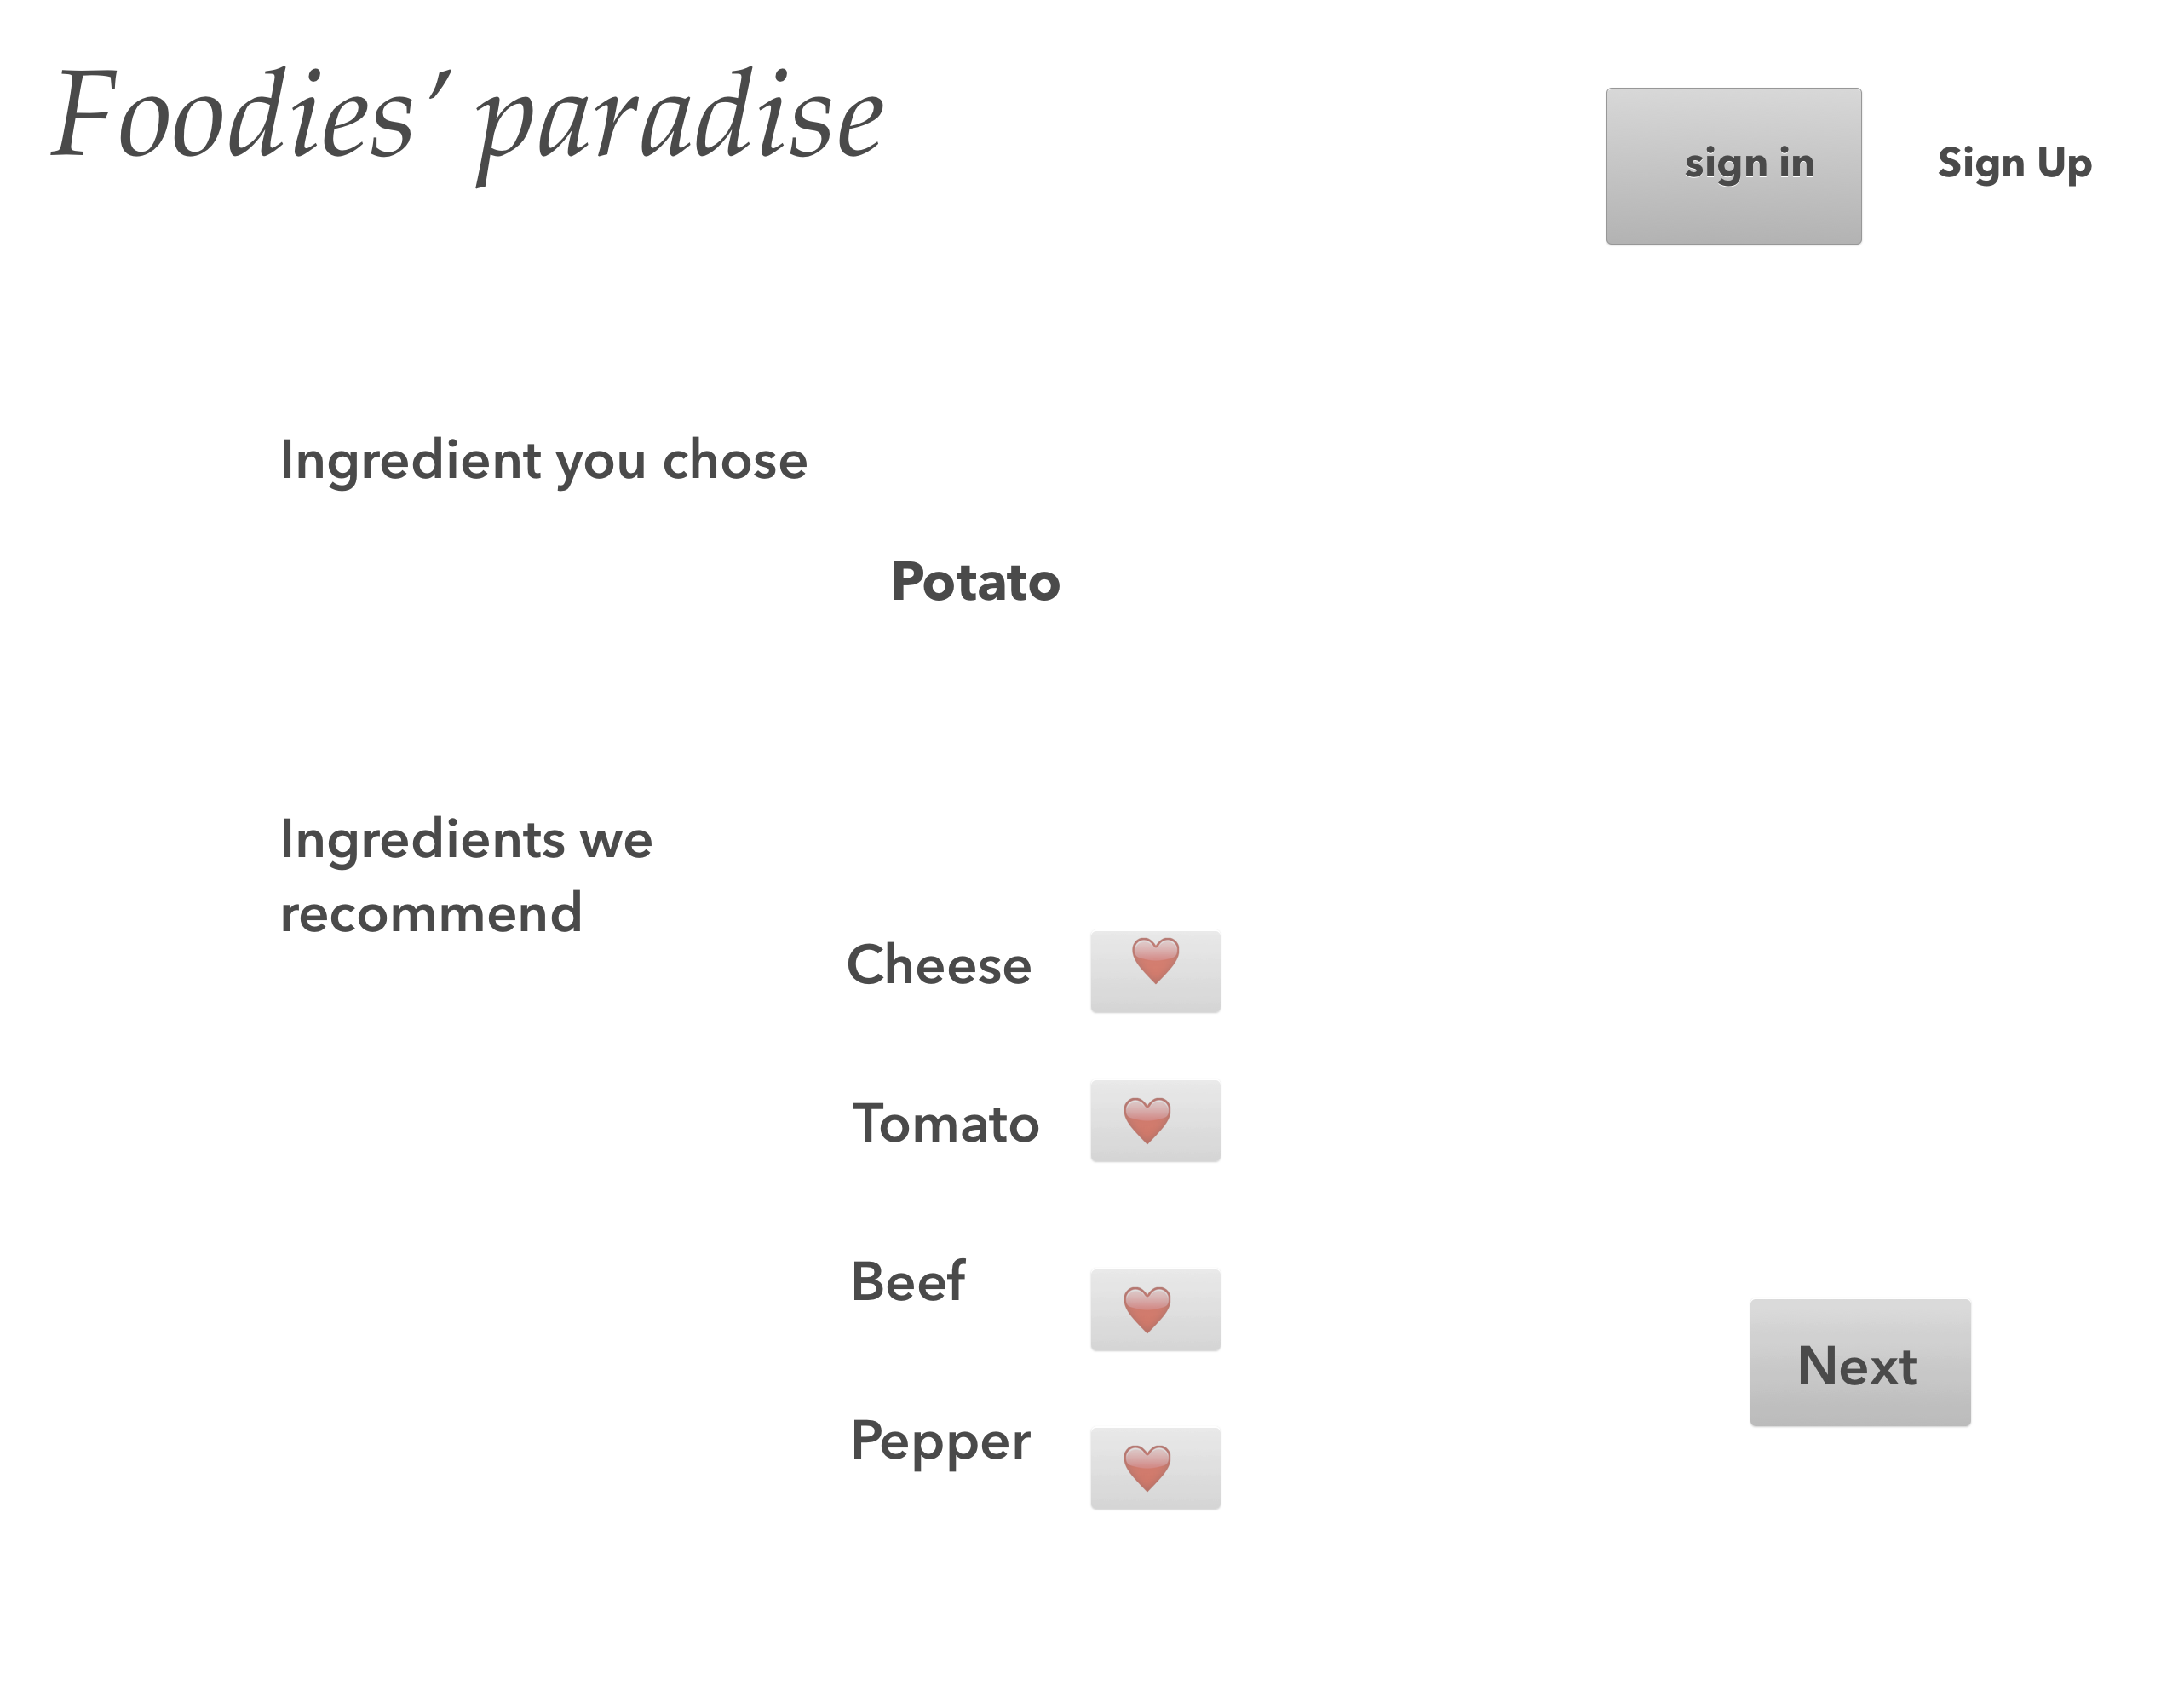
\includegraphics[width=.48\textwidth]{ui_3}} \\
\\
\\
\frame{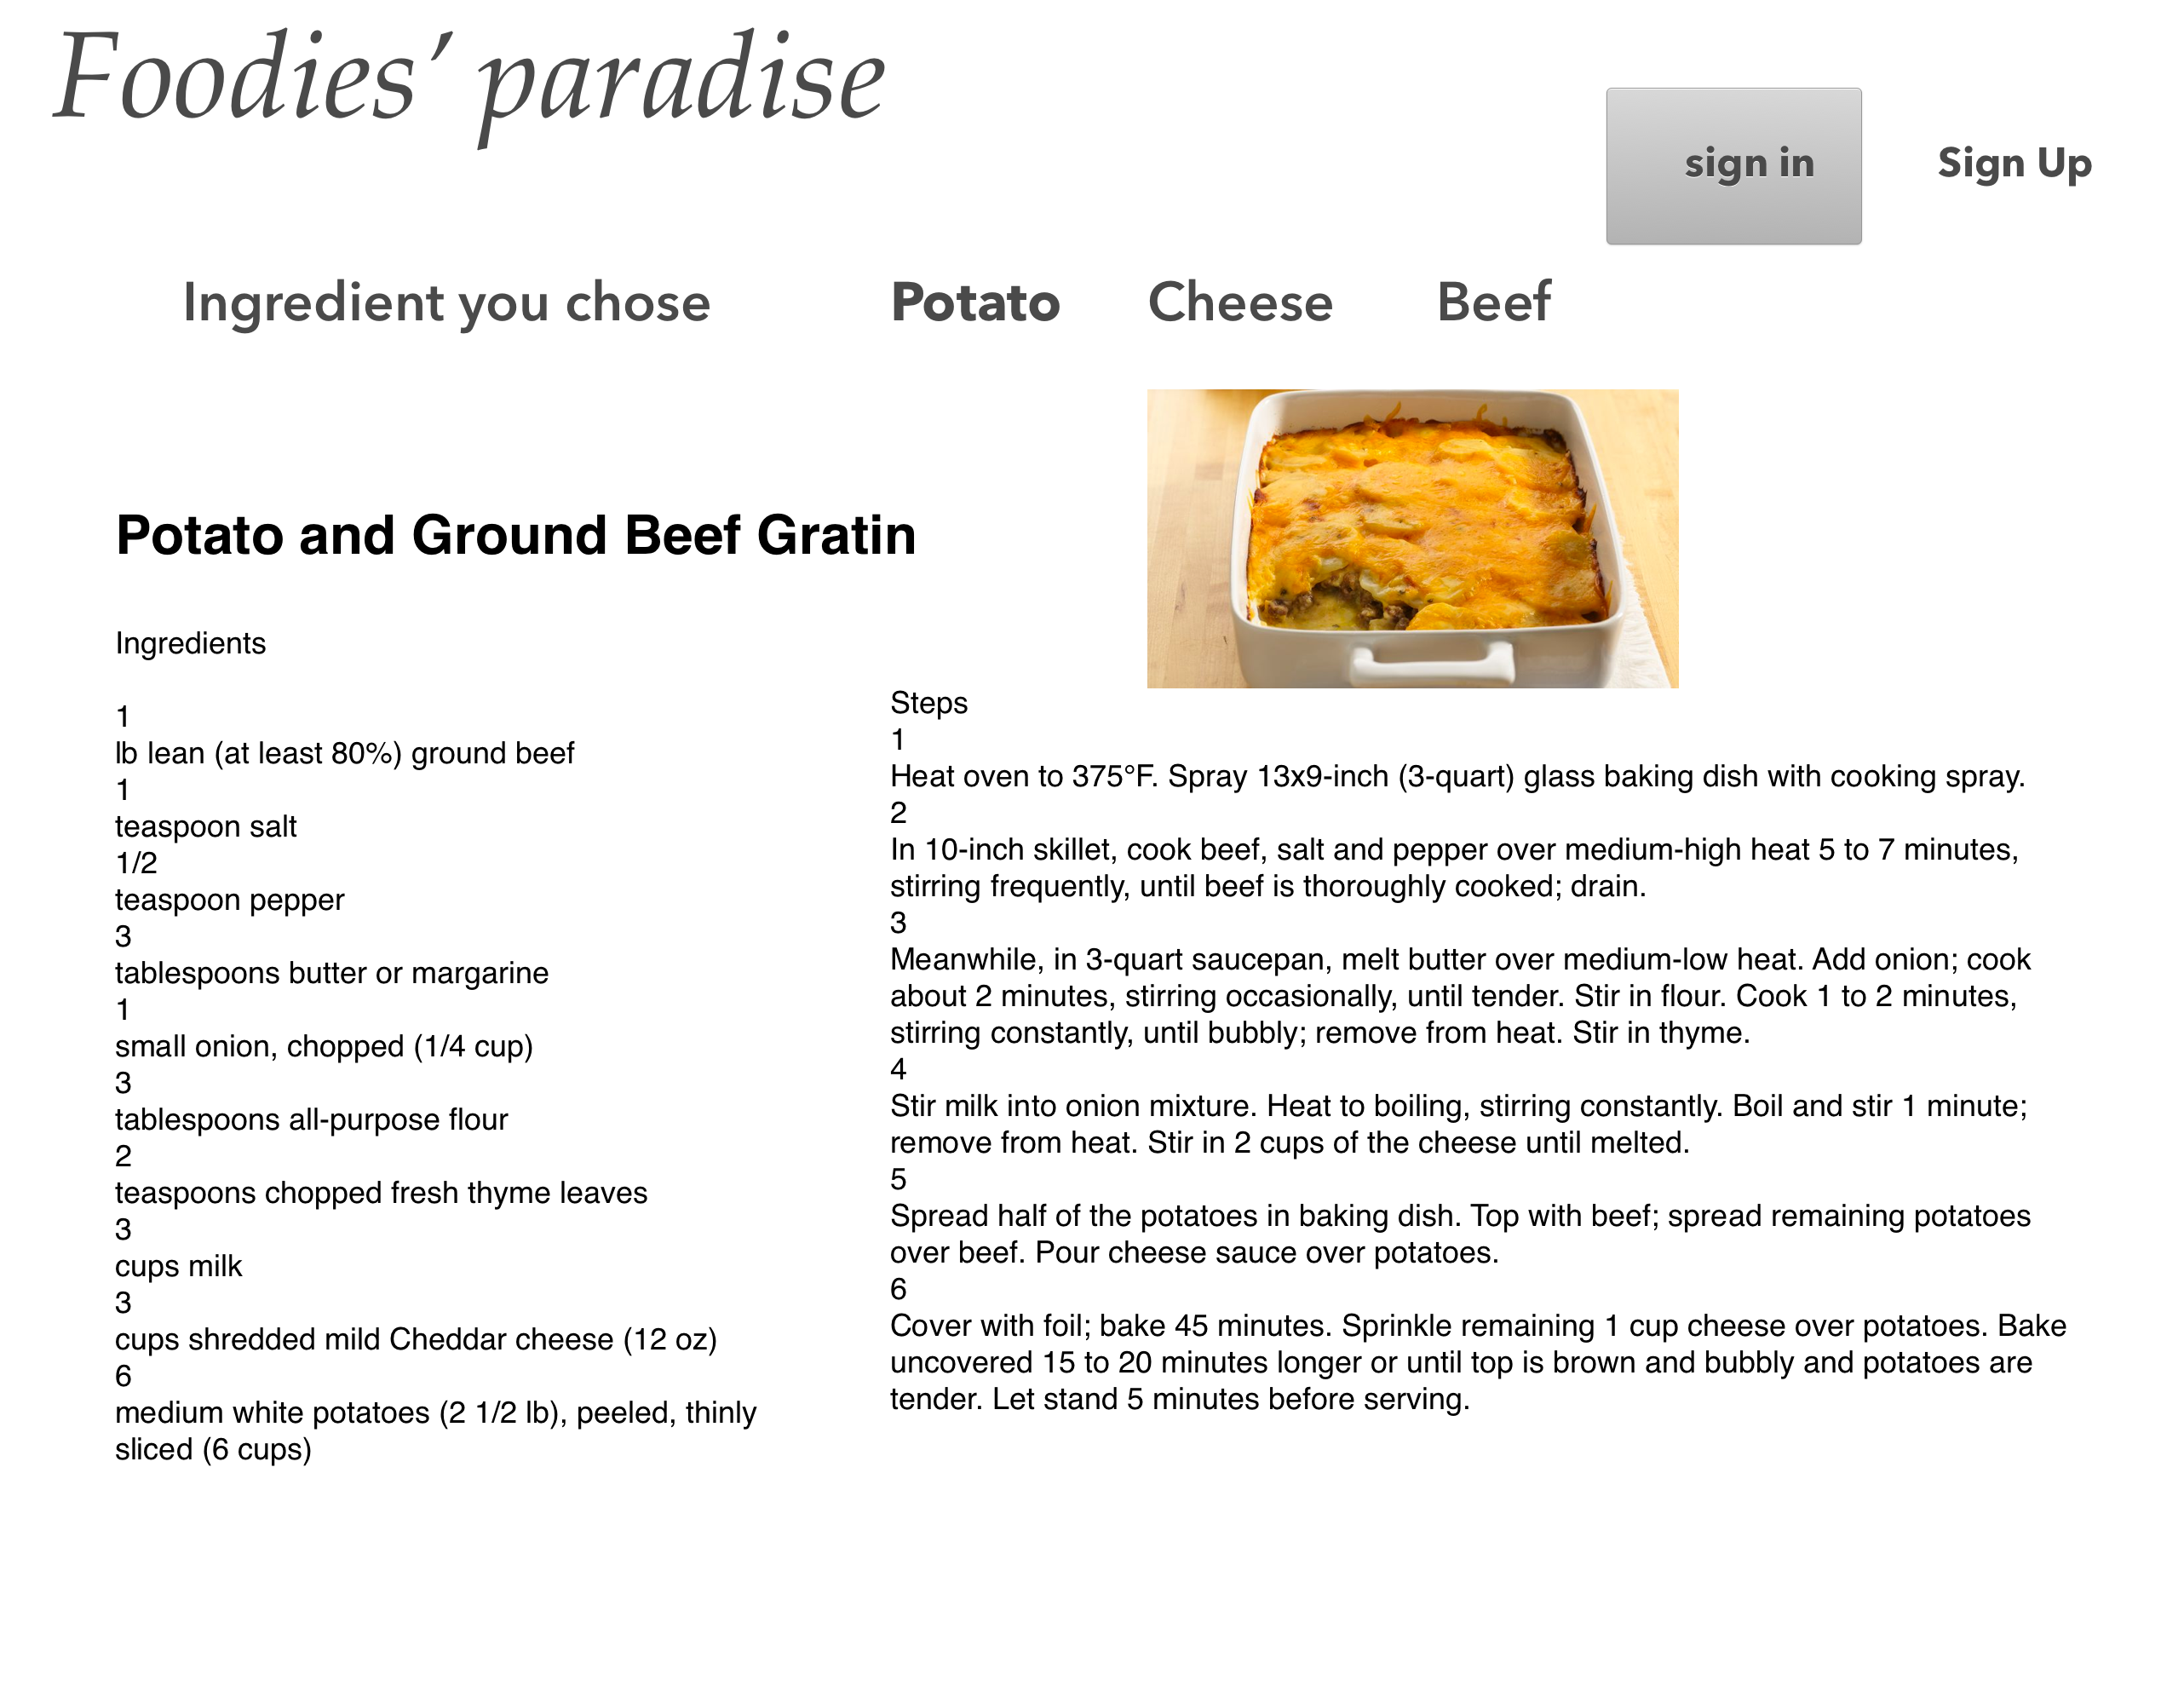
\includegraphics[width=.48\textwidth]{ui_4}} \\

\section{Preliminary Results and Analysis}
The preliminary results our group obtained are the co-occurrence network and flavor network, based on which we could achieve a reasonable recommendation of ingredients and recipes for the user. In particular, our group managed to recommend four ingredients given an input ingredient based on co-occurrence network and flavor analysis to the user, and therefore we can generate a recipe based on those ingredients.\cite{restle1955theory}\\
\indent Below is an example of the result, with the first line being the queries, and the corresponding 4 recommendations. 

\begin{table}[H]
\begin{center}
\begin{tabular}{ c c c c}
Shrimp&Beef&Egg&Tomato\\
\hline
Clam&Carrots&Cottage&lettuce\\
Squid&Beef Broth&Bread Crumbs&Pita\\
Mussels&Onion&Fat Free Ricotta Cheese&Okra\\
Clam Juice&Veal&Ricotta Cheese&Seafood\\
\end{tabular}
\caption{Time Line}
\end{center}
\end{table}

The problem with our current algorithm is, the recommended ingredients may be too uncommon to give recipe recommendations. Also without tagging for recipes and ingredients, the recommendation may not satisfy users’ need.\\


\section{Design of Upcoming Experiments}
Our group will adjust the number of ingredients obtained after the filtration using flavor table. Instead of using four final ingredients, five, six or even more ingredients could be used to be shown to the user to cover more ingredients.\\
\indent Our group will experiment by adding tags to the recipes or ingredients to achieve a more purposeful recommendation. In particular,  we can give recommendations of ingredients and recipes based on users’ selected dish type and ingredient type.\\
\indent We need to filter out uncommon ingredients when giving recommendation on ingredients. Therefore we have more flexibility when giving recipe recommendations.\\ 

\section{List of Innovations}
Unlike popular recipe recommendation systems that either rely on ingredient frequencies or user ratings, we aim to integrate the two approaches and interpret the results with favor compounds analysis, which also allows us to generate customized recipes.\\
\indent Since we are using flavor similarity between each two ingredients to give recommendation, we proposed a series of innovation recommendation methods that using flavor information. 1. We tried to use flavor similarity to substitute ingredients. 2. We tried to use flavor similarity as a threshold when recommending other ingredients to generate the recipe.\\

\section{Conclusions and Discussion} 
We believe that with further modifications and ameliorations based on our proposed upcoming experiments, the recommendation system will give better results for the user and the user interface to be built on the system will be easy and convenient to use.\\

\section{Project Planning}

Original Planning and Task Assignmnets (Table 1 and Table 2):
\begin{table}[H]
\begin{center}
\begin{tabular}{ c c }
Time & Task  \\ 
 \hline
Oct 16th & Gather and clean data\\
Oct 20th &Build data model\\
Oct 30th &Demo \\
Nov 6th &Build UI\\
Nov 10th &Progress report \\
Nov 13th &Add data analysis component \\
Nov 20th &Add user interactive function\\
Nov 27th &Improve features and functions\\
12/5 &Final report \\
\end{tabular}
\caption{Time Line}
\end{center}
\end{table}

\begin{table}[H]
\begin{center}
\begin{tabular}{ c c c c c c c }
Task & Siyi & Mo & Sixin & Jidong & Haiyue & Shan\\
\hline
Proposal &\checkmark &\checkmark &\checkmark &\checkmark &\checkmark &\checkmark\\
Data Collection &\circle &\circle & &\circle & &\circle\\
Data Cleaning & &\circle &\circle &\circle & &\\
UI &\circle & & & &\circle &\\
Database & & &\circle & &\circle &\circle\\
Analysis &\circle &\circle & &\circle &\circle &\\
Test & & \circle&\circle & & &\circle\\
Finalization &\circle &\circle &\circle &\circle &\circle &\circle\\
\end{tabular}
\caption{Task Assignments}
\end{center}
Note: \checkmark Completed \circle Assigned
\end{table}
New Planning and Task Assignmnets (Table 3 and Table 4):
\begin{table}[H]
\begin{center}
\begin{tabular}{ c c }
Time & Task  \\ 
 \hline
Nov 15th &Add data analysis component \\
Nov 20th &Build UI\\
Nov 23rd &Add user interactive function \\
Nov 27th &Improve features and functions\\
Dec 5th &Final report \\
\end{tabular}
\caption{Time Line}
\end{center}
\end{table}

\begin{table}[H]
\begin{center}
\begin{tabular}{ c c c c c c c }
Task & Siyi & Mo & Sixin & Jidong & Haiyue & Shan\\
\hline
Proposal &\checkmark &\checkmark &\checkmark &\checkmark &\checkmark &\checkmark\\
Data Collection &\checkmark &\checkmark & &\checkmark & &\checkmark\\
Data Cleaning & &\checkmark &\checkmark &\checkmark & &\\
UI &\circle & & & &\circle &\\
Database & & &\checkmark & &\checkmark &\checkmark\\
Analysis &\checkmark &\checkmark & &\checkmark &\checkmark &\\
Test & & \circle&\circle & & &\circle\\







Finalization &\circle &\circle &\circle &\circle &\circle &\circle\\
\end{tabular}
\caption{Task Assignments}
\end{center}
Note: \checkmark Completed \circle Assigned
\end{table}

\textbf{Notes:} All team members contributed similar amount of effort.

\bibliographystyle{ACM-Reference-Format}
\bibliography{reference.bib} 

\end{document}
